\documentclass{article}
\usepackage{color}
\usepackage{soul}
\usepackage{multirow}
\usepackage{pgfplots}
\usepackage{ifthen}
\usepackage[UTF8]{ctex}
\usepackage[left=3.0cm,right=3.0cm,top=2.5cm,bottom=2.5cm]{geometry}
\geometry{a4paper}
\usepackage{tikz}
\usetikzlibrary{chains}
\newcommand{\diff}{\mathop{}\!\mathrm{d}}
\usepackage{appendix} 
\usepackage{lipsum}
\usepackage{listings}
\usepackage{diagbox}
\usepackage{pdfpages}
\usepackage{xcolor}
\usepackage{pdflscape}
\usepackage{soul}
\usepackage{booktabs}
\usepackage{longtable}
\usepackage[most]{tcolorbox}
\newtcolorbox{mycolorbox}[1][]{
  sharp corners,
  colback=white, 
  colframe=black, 
  coltext=blue, 
  boxsep=5pt, 
  left=2pt, 
  right=2pt, 
  top=1pt, 
  bottom=1pt,
  breakable,
  #1 
}
\usepackage{subcaption}
\lstset{
    backgroundcolor=\color{gray!20},
    basicstyle=\ttfamily,
    commentstyle=\color{darkgray}\ttfamily,
    stringstyle=\color{red},
    showstringspaces=false,
    numbers=left,
    numberstyle=\tiny\color{gray},
    stepnumber=1,
    numbersep=10pt,
    tabsize=4,
    showspaces=false,
    showtabs=false,
    frame=single,
    captionpos=b,
    breaklines=true,
    breakatwhitespace=false,
    escapeinside={\%*}{*)},
    breaklines=true,
    xleftmargin=\parindent,
    xrightmargin=\parindent,
}
\lstdefinestyle{dockerstyle}{
    language=bash,
    keywordstyle=\color{blue}\bfseries,
    morekeywords={FROM, RUN, CMD, LABEL, EXPOSE, ENV, ADD, COPY, ENTRYPOINT, VOLUME, USER, WORKDIR, ARG, ONBUILD},
}
\lstdefinestyle{pythonstyle}{
    language=Python,
    keywordstyle=\color{blue}\bfseries,
    morekeywords={import, from, as, def, return, class, self, if, elif, else, while, for, try, except, with},
}
\lstdefinestyle{cstyle}{
    language=C,
    keywordstyle=\color{blue}\bfseries,
    morekeywords={size_t, printf}, 
}
\lstdefinestyle{bashstyle}{
    language=bash,
    keywordstyle=\color{blue}\bfseries,
    morekeywords={echo,sudo ,if, then, else, fi, for, in, do, done, echo, exit, return, function},
    commentstyle=\color{green}\ttfamily,
}
\usepackage{algorithm}
\usepackage{algpseudocode}
\renewcommand{\algorithmicrequire}{\textbf{Input:}}  
\renewcommand{\algorithmicensure}{\textbf{Output:}}  
\usepackage{amsmath}
\usepackage{amsthm}
\DeclareMathOperator{\sigm}{sigm}
\usepackage{graphicx}
\usepackage{float}
\renewcommand{\vec}[1]{\boldsymbol{#1}}
\usepackage{amssymb}
\usepackage{booktabs} 
\usepackage{hyperref}
\usepackage{titlesec}
\usepackage{caption}
\usepackage{fontspec}
\usepackage{xeCJK}
\setCJKmainfont{SimSun} 
\title{\Huge 数据库(2)实验2}
\author{21121178 王士博}
\begin{document}
\begin{center}
    \textbf{\huge 数据库(2)实验3:HDFS分布式文件系统和SparkSQL实验}
\end{center}
\begin{center}
    \textbf{\large \textbf{学号:21121178 \quad 姓名:王士博 \quad 指导教师:刘洋}}
\end{center}
\hrulefill
\section{实验环境}
\begin{itemize}
    \item 腾讯云服务器配置:竞价实例,香港地区,标准型SA5,8核 16GB,Ubuntu 20.04。
\end{itemize}
\section{实验目的}
\begin{enumerate}
    \item 了解Docker和Kubernetes的安装和使用方法。
    \item 学会创建镜像和实现实例克隆。
    \item 学会创建Kubernetes集群,部署服务和实例,验证Kubernetes的负载均衡和快扩容和快恢复特性。
\end{enumerate}
\section{实验步骤}
\subsection{生成安装所有依赖的镜像}
\begin{enumerate}
    \item 安装JDK8和JRE(其实直接安装JDK会包括JRE),使用\texttt{apt-get}安装之后需要在\texttt{.bashrc}
    中显示给出\texttt{JAVA\_HOME}的路径,并且使用\texttt{source}应用更改。
    \begin{figure}[H]
        \centering
        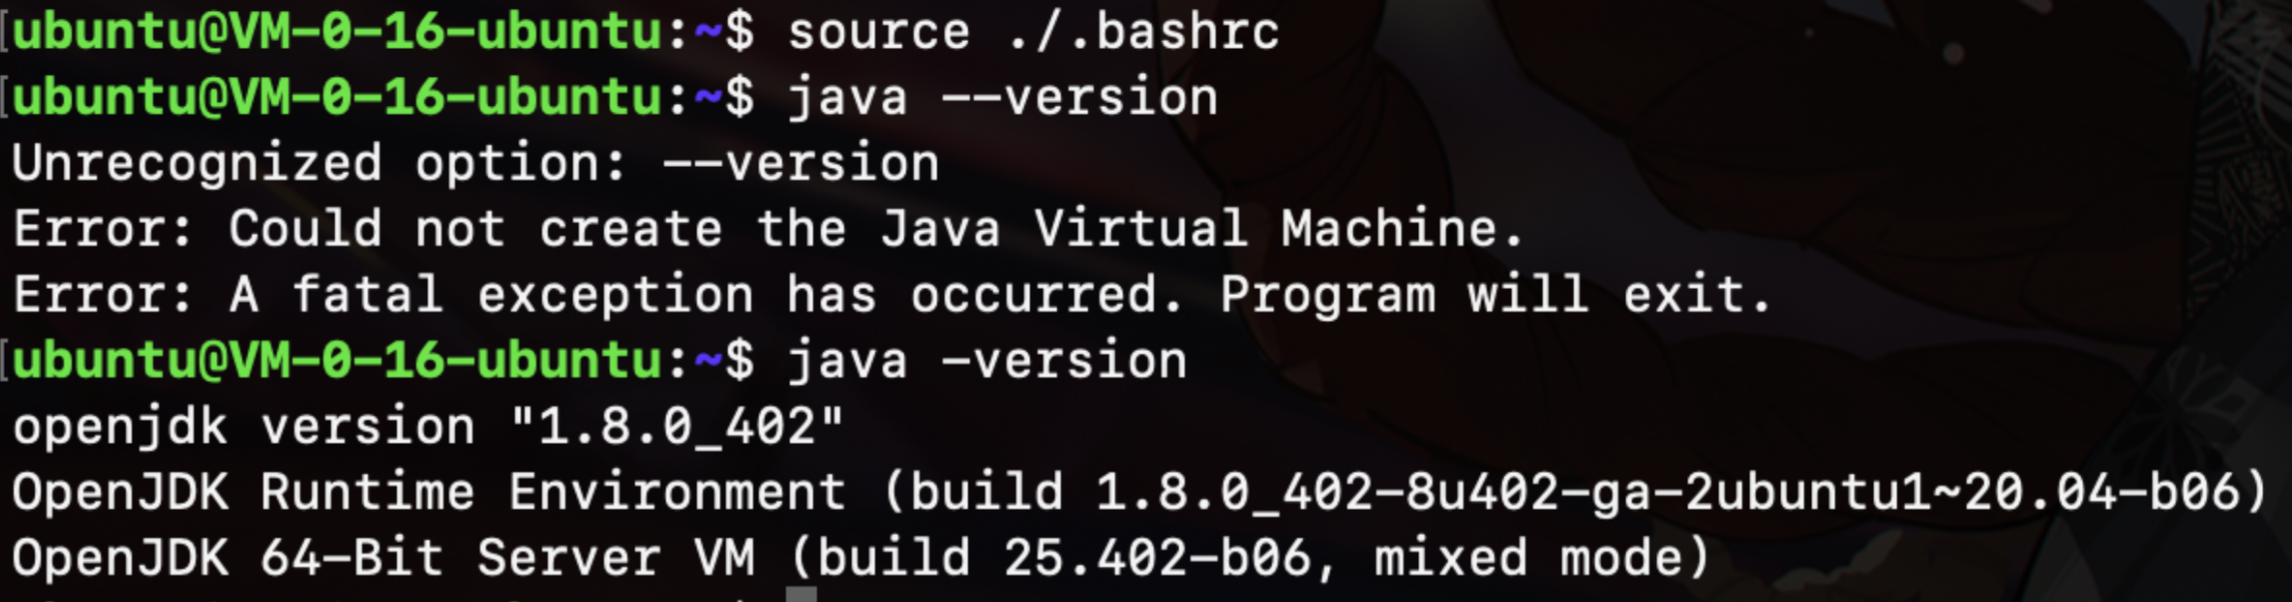
\includegraphics[width=0.7\textwidth]{java.png}
    \end{figure}
    \item 使用scp上传本地的Hadoop和Spark压缩包到服务器并且解压到软件包目录\texttt{/usr/local/}下
    ,更改文件的owner为当前的用户,并且赋予所有的权限,然后cd进可执行文件使用\texttt{-version}来测试
    Hadoop安装包的完整性以及安装的成功性,并且使用\texttt{SparkPi}来测试Spark的安装成功性。
    \begin{figure}[H]
        \begin{subfi
    \end{figure}
    \begin{figure}[H]
        \centering
        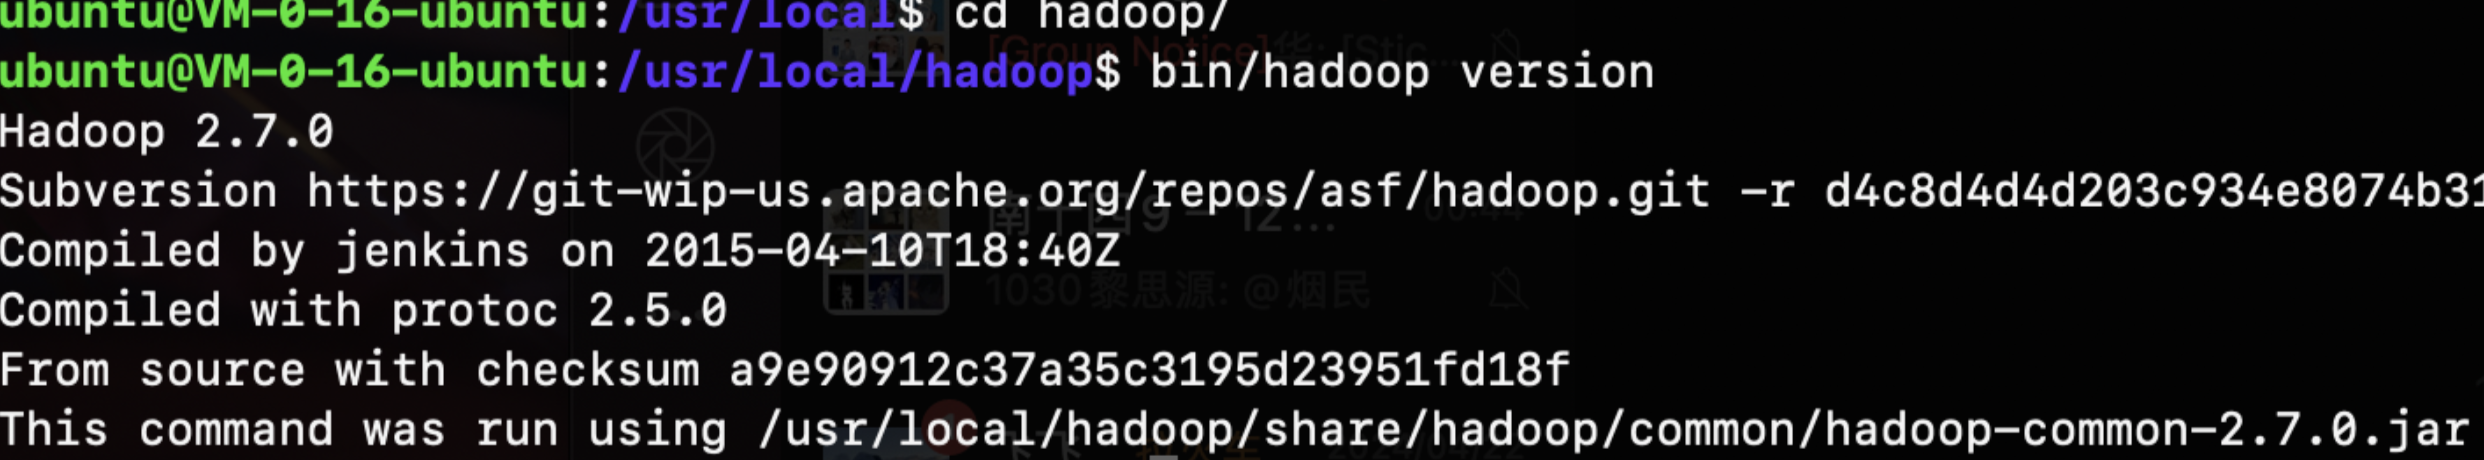
\includegraphics[width=0.65\textwidth]{hadoopinstall.png}
    \end{figure}
    \begin{figure}[H]
        \centering
        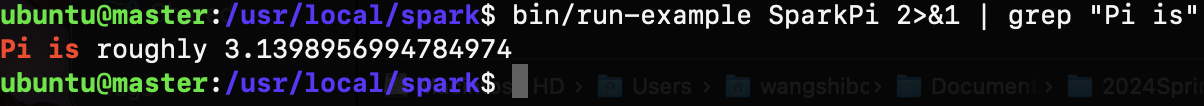
\includegraphics[width=0.5\textwidth]{sparkpi.png}
    \end{figure}
    \item 
\end{enumerate}
\subsection{创建三个实例启动分布式文件系统HDFS}

\subsection{Titanic数据集的分析}

\section{实验结论}

\end{document}